\subsection{W-SN-DCGAN}
\label{sec:exp-wsndcgan}
We replace weight clipping by spectral normalization. A first experiment with the same hyper-parameters as for all other models has shown very poor performance. By further looking into the literature, we found out that when using an optimizer such as Adam, setting $\beta_1$ (the exponential decay rate for the first moment estimate) to 0 was recommended when using the Wasserstein loss \cite{arjovsky2017wasserstein}.

The evolution of the Inception score and losses is reported in Figures \ref{fig:exp-w-sn-dcgan-is} and \ref{fig:exp-w-sn-dcgan-losses}. We observe stable Inception score and loss evolution, compared to the previous methods. We note that the generator loss is inverted compared to that of the SN-DCGAN, that is simply because of the different formulation of the loss. However, the Inception score does not seem to reach significantly higher values than with the SN-DCGAN.

\begin{figure}[H]
    \centering
    \begin{subfigure}[t]{0.49\textwidth}
        \centering
		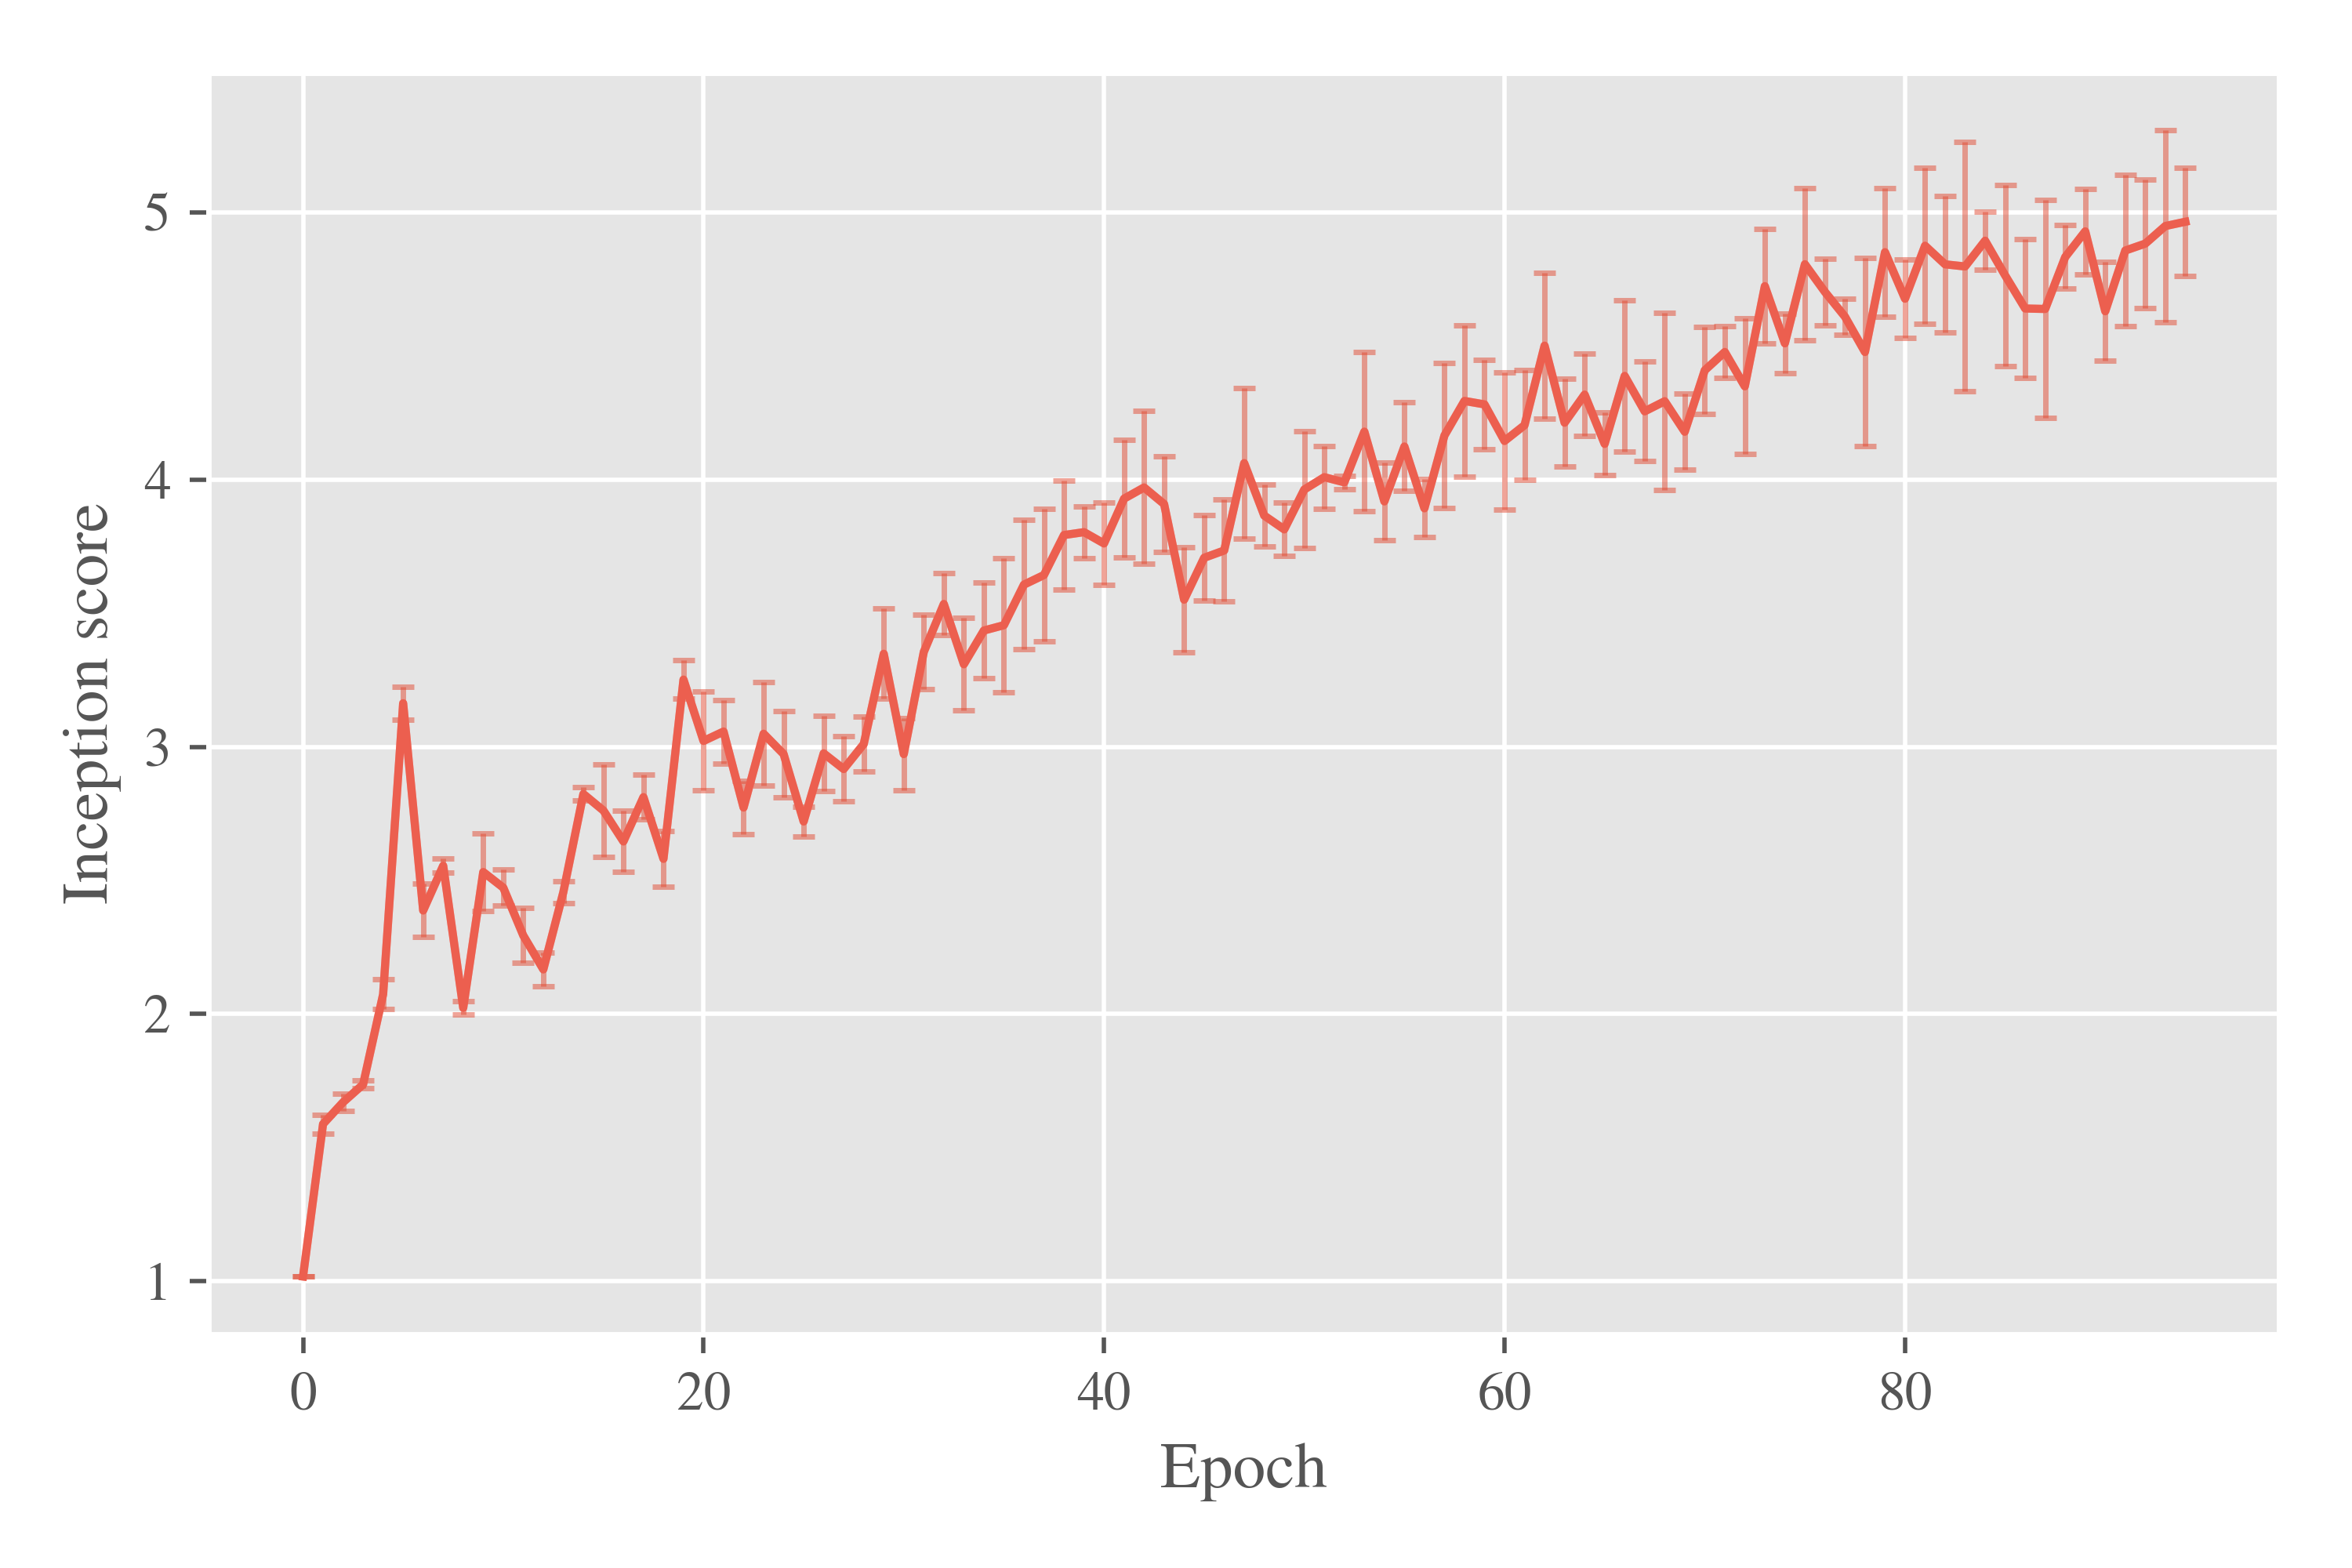
\includegraphics[width=\textwidth]{../code/results/figures/w-sn-dcgan_cifar10_is.png}
		\caption{Inception score\\~}
		\label{fig:exp-w-sn-dcgan-is}
    \end{subfigure}
    \begin{subfigure}[t]{0.49\textwidth}
        \centering
        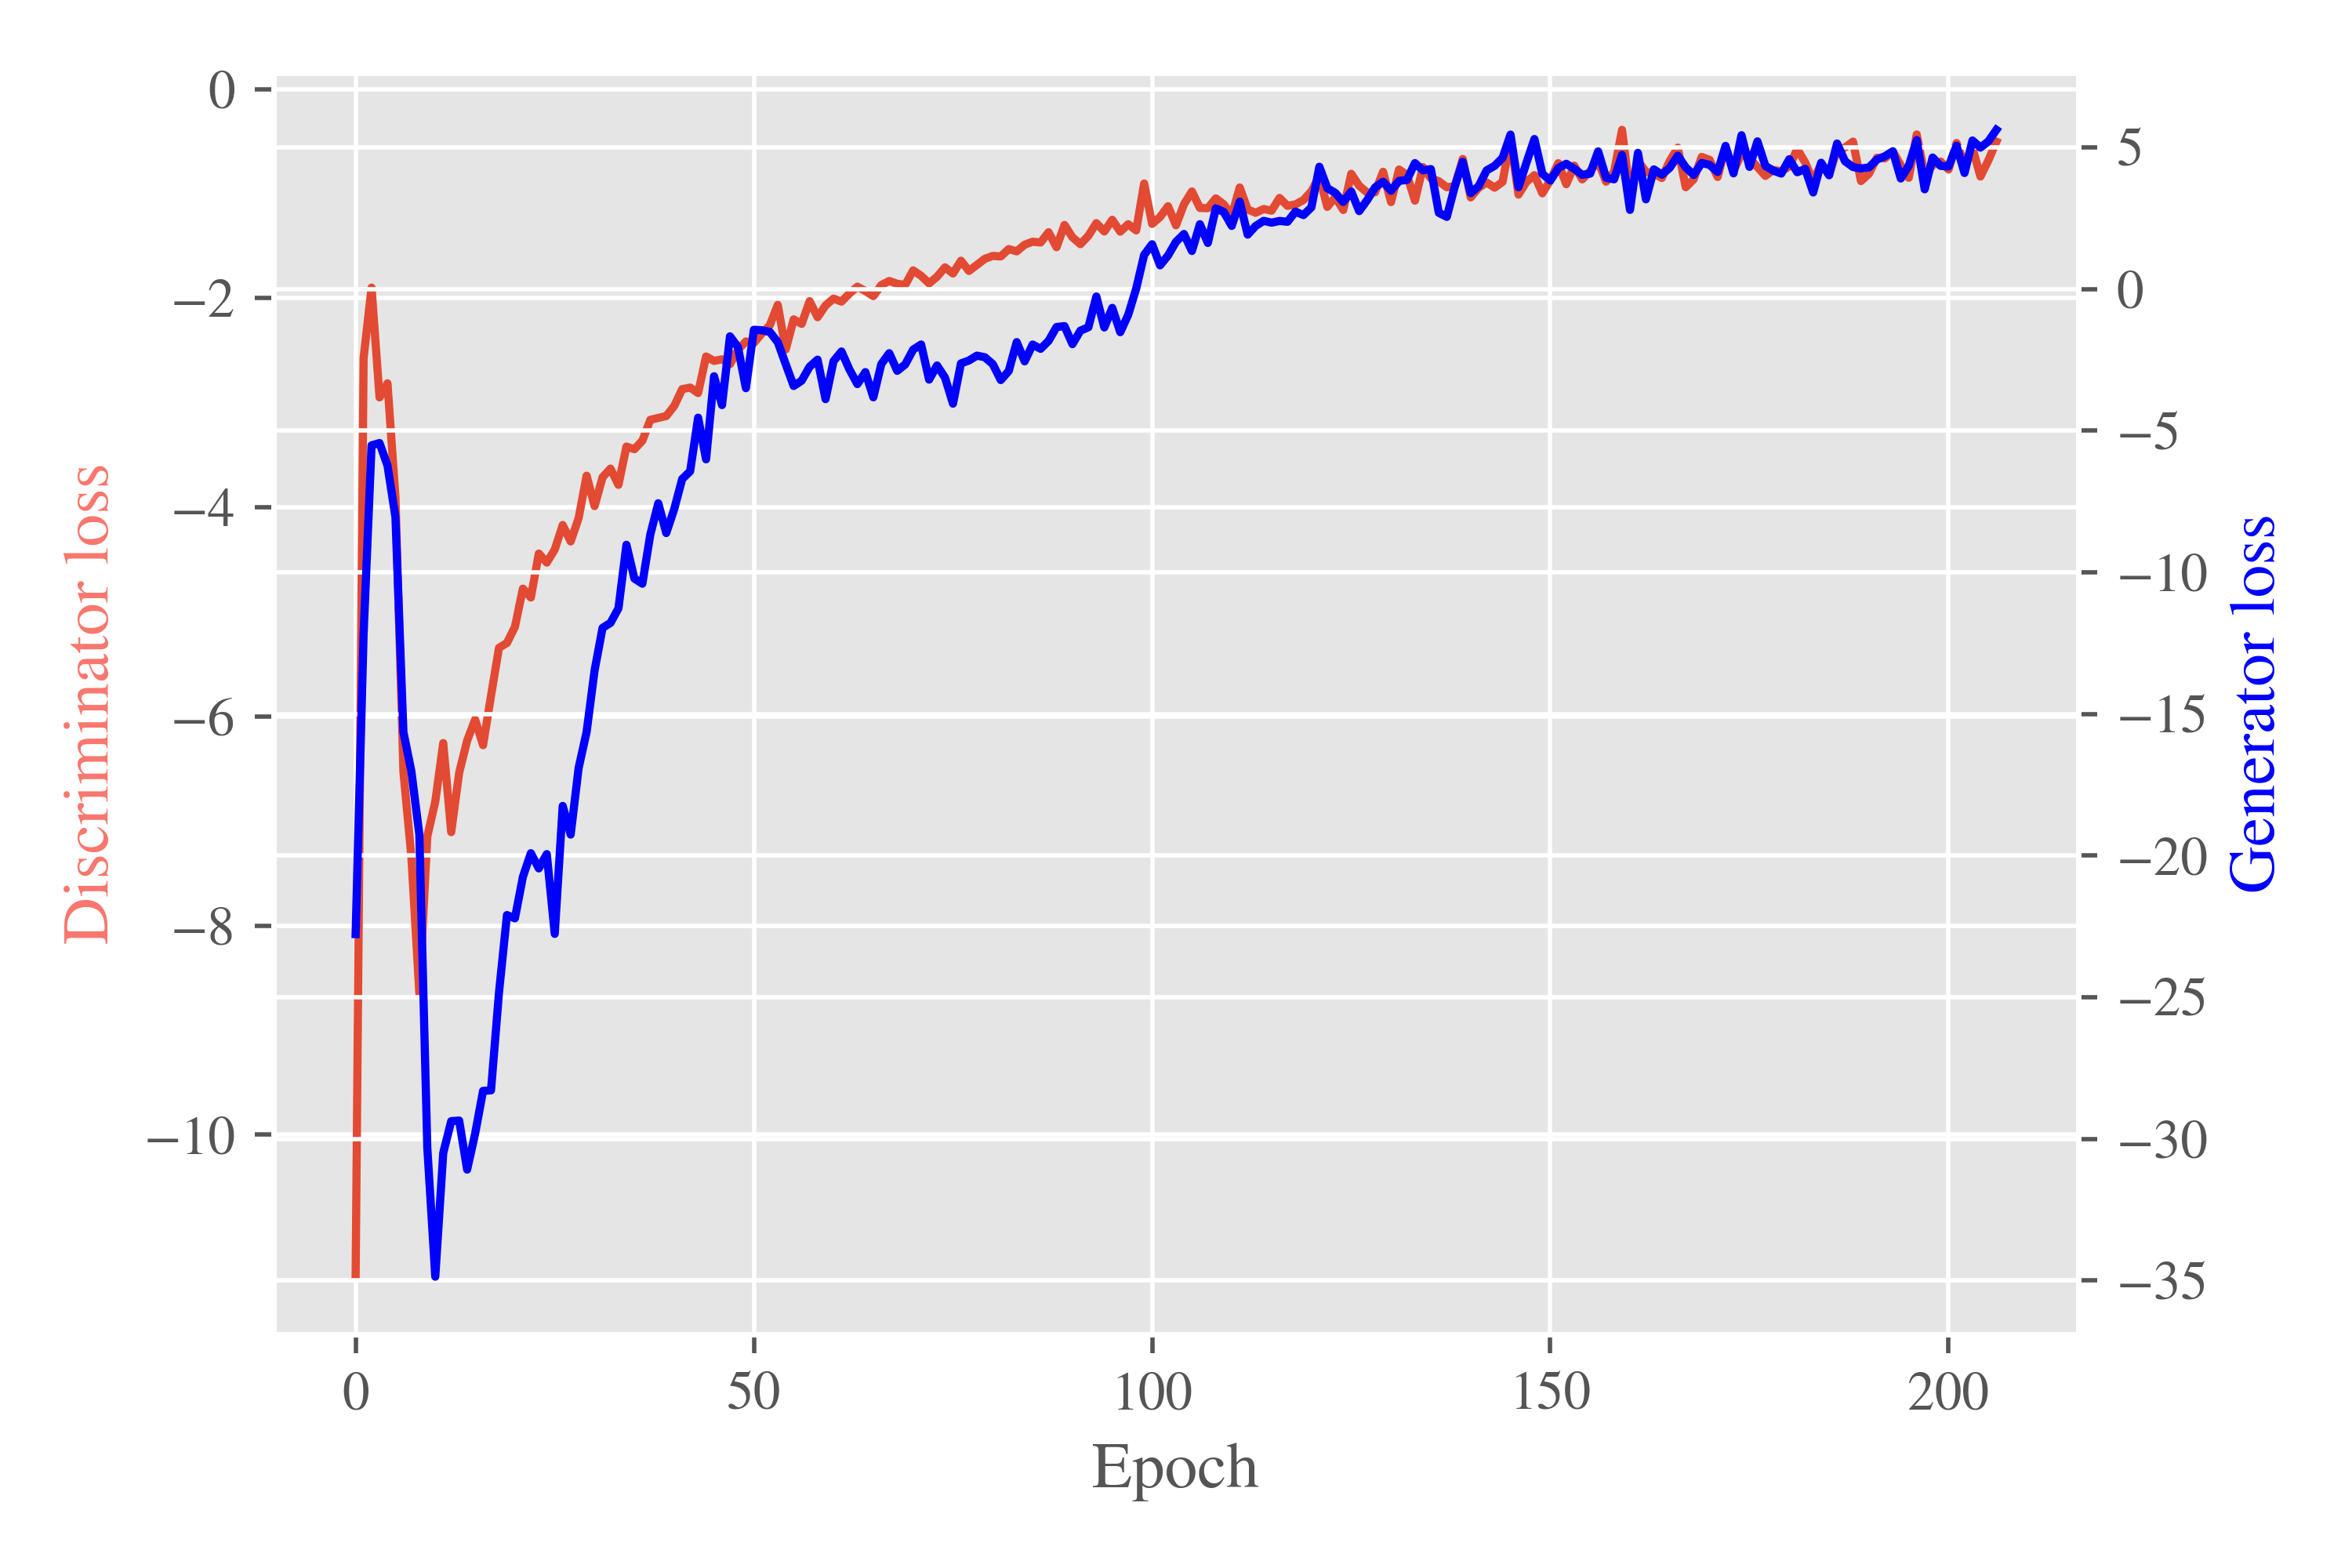
\includegraphics[width=\textwidth]{../code/results/figures/w-sn-dcgan_cifar10_losses.png}
		\caption{Losses\\~}
		\label{fig:exp-w-sn-dcgan-losses}
    \end{subfigure}
    \caption{W-SN-DCGAN - training on CIFAR10 over 200 epochs.}
\end{figure}

We show example generations on both of our datasets:
\begin{figure}[H]
\centering
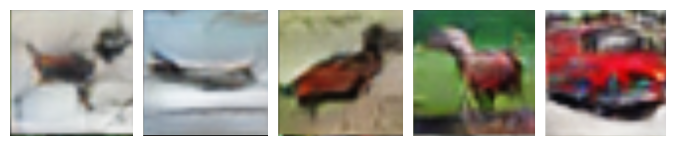
\includegraphics[width=0.7\textwidth]{../code/results/figures/images/w-sn-dcgan_cifar10}
\caption{W-SN-DCGAN - generated images after training on CIFAR10.}
\end{figure}

\begin{figure}[H]
\centering
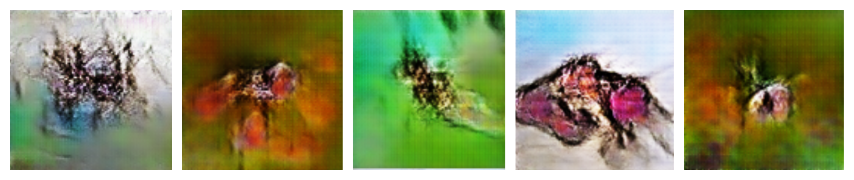
\includegraphics[width=0.7\textwidth]{../code/results/figures/images/w-sn-dcgan_reptiles}
\caption{W-SN-DCGAN - generated images after training on Reptiles. We could not train for a sufficient time; these images show usual signs of the early stages of GAN training, e.g. repetitive patterns within the image and unclear object.}
\end{figure}